\documentclass[11pt]{article}

\usepackage{CMPSC465}
\usepackage{enumitem}
\usepackage{algpseudocode}
\usepackage{tikz}
\usepackage{CMPSC465}
\usepackage{enumitem}
\usepackage{algpseudocode}
\usepackage{tikz}
\usepackage{amsmath}
\usepackage{tikz} 
\usepackage{graphicx}
\usepackage[colorlinks=true, allcolors=blue]{hyperref}
\usepackage{tkz-graph}
\PassOptionsToPackage{usenames,dvipsnames,svgnames}{xcolor}  
\usepackage{tikz}
\usetikzlibrary{arrows,positioning,automata}

\def\title{Assignment 06}

\def\defeq{\mathrel{\mathop:}=}
%\usepackage{algpseudocode}
%\usepackage{algorithm}
\usepackage[ruled,noline]{algorithm2e}
%\usepackage{amsthm}
\newcommand\nonl{%
  \renewcommand{\nl}{\let\nl\oldnl}}% Remove line number for one line
  
\newcommand{\aaa}[1]{\hspace{0.65cm}\parbox[t]{15.3cm}{#1}}
\newcommand{\aab}[1]{\hspace{1.15cm}\parbox[t]{15.0cm}{#1}}
\newcommand{\aac}[1]{\hspace{1.65cm}\parbox[t]{15.0cm}{#1}}
\newcommand{\aad}[1]{\hspace{2.15cm}\parbox[t]{15.0cm}{#1}}
\newcommand{\aaA}[2]{\hspace{0.5cm} {\tikz[overlay] \draw (0.1, -0.1) -- (0.1, #1 * -1.5em + 0.6em);} \parbox[t]{15.0cm}{#2}}
\newcommand{\aaB}[2]{\hspace{1.0cm} {\tikz[overlay] \draw (0.1, -0.1) -- (0.1, #1 * -1.5em + 0.6em);} \parbox[t]{15.0cm}{#2}}
\newcommand{\aaC}[2]{\hspace{1.5cm} {\tikz[overlay] \draw (0.1, -0.1) -- (0.1, #1 * -1.5em + 0.6em);} \parbox[t]{15.0cm}{#2}}
\newcommand{\aaD}[2]{\hspace{2.0cm} {\tikz[overlay] \draw (0.1, -0.1) -- (0.1, #1 * -1.5em + 0.6em);} \parbox[t]{15.0cm}{#2}}
\newcommand{\xxx}{\par\vspace{0.1cm}}

\begin{document}
\maketitle

\section*{Due: Friday 11:59 pm, Feb.\ 25, 2022}

\paragraph*{Instructions:}

You may work in groups of up to three people to solve the homework.
You must write your own solutions and explicitly acknowledge everyone whom 
you have worked with or who has given you any significant ideas about your solutions. 
You may also use books or online resources to help solve homework problems.  
All consulted references must be acknowledged. The acknowledgements need to be made by answering Problem~1 below.

You are encouraged to solve the problem sets on your own using only the textbook and lecture notes as a reference. This will give you the best chance of doing well on the exams. Relying too much on the help of group members or on online resources will hinder your performance on the exams.

Submissions being late in 2 hours will be accepted with a 20\% penalty. Submissions late more than 2 hours will receive 0. There will be no exceptions to this policy, as we post the solutions soon after the deadline. 

For the full policy on assignments, please consult the syllabus.

\paragraph*{Formatting:} Start a new page for each problem.

\paragraph*{Describing an Algorithm:} Please make sure you use plain wording to explain your algorithm. It is always a good practice to start with a summary of the high-level idea of your algorithm to ease graders understand your solution quickly. Then, explain your algorithm, using plain wording and including enough details.

The use of pseudo-code is optional, and it is your decision. No matter you use it or not, above description in words is always required. The pseudo-code has its own advantage in explaining structured (i.e., if-else, for-loop, recursive functions, etc) algorithms and in putting details in the right place. If you think pseudo-code better explains your algorithm, and/or helps graders understand your solution, and/or contains more details not included in the plain-wording description, then use pseudo-code. If you think everything is already clearly explained in the description with words, then you don't need to include pseudo-code. An algorithm that is only written in pseudo-code (i.e., missing above plain-wording description) is not acceptable, as it is extremely hard to read just pseudo-code without any explanation.

Here is a general situation that may help you decide whether to use pseudo-code or not. An algorithm could be ``designed from scratch'', i.e., you will need to come up with the step-by-step procedure. This usually involves in implementing a function with clear input and output. In this case, including pseudo-code usually helps. All algorithm we've seen so far (e.g., merge-two-sorted-arrays, merge-sort, etc) falls in this category. Second, an algorithm could also be ''transformed into another algorithm'', i.e., you use an existing algorithm to solve this problem. In this case you usually don't need to include pseudo-code but to describe how to transform one problem into the other. We will see such examples soon.

\clearpage\newpage

\begin{qunlist}
\setcounter{sparectr}{-1}

\q{0}{Acknowledgements. }
	The assignment will receive a 0 if this question is not answered.
\begin{enumerate}
	\item If you worked in a group, list the members of the group. Otherwise, write ``I did not work in a group.''
	\item If you received significant ideas about your solutions from anyone not in your group, list their names here. Otherwise, write ``I did not consult  anyone except my group members''.
	\item List any resources besides the course material that you consulted in order to solve the material. If you did not consult anything, write ``I did not consult any non-class materials.''
\end{enumerate}

\q{10}{} Consider this algorithm to find all connected components of a directed
graph $G$: run DFS-with-timing on $G$ to get the postlist~(\textcolor{blue}{i.e., the list of vertices in decreasing post value}),
and then use the reverse of the postlist as a ``magic ordering'' to run the DFS algorithm \textcolor{blue}{on graph $G$}.
Design an instance to demonstrate that this algorithm is incorrect.
Specifically, you will need to give a directed graph, then run above algorithm
and show that the resulting $visited$ array does not give the correct connected
components of $G$. 


% Qimin
\q{10}{}
%\begin{enumerate}
%\item Given an undirected graph $G = (V, E)$, a vertex $t \in V$, and an edge $e = (u,v)\in E$, design a $O(|V|+|E|)$ time algorithm to determine whether there exists a cycle in $G$ that contains both $t$ and $e$.
Given a directed graph $G = (V, E)$, a vertex $t \in V$, and an edge $e = (u,v)\in E$, design
an $O(|V|+|E|)$ time algorithm to determine whether there exists a cycle in $G$ that contains both $t$ and $e$.
%\end{enumerate}


% Tianyang
\q{10}{} Design an algorithm runs in $O(|V| + |E|)$ time which takes a directed graph as the input and determines if there is a vertex such that all other vertices are reachable from it.

% Manohar
\q{12}{} Run the algorithm to determine connected components on the following
directed graphs $G$. When doing DFS on the reverse-graph $G^R$, whenever there is a choice of
vertices to explore, always pick the one that is alphabetically first.

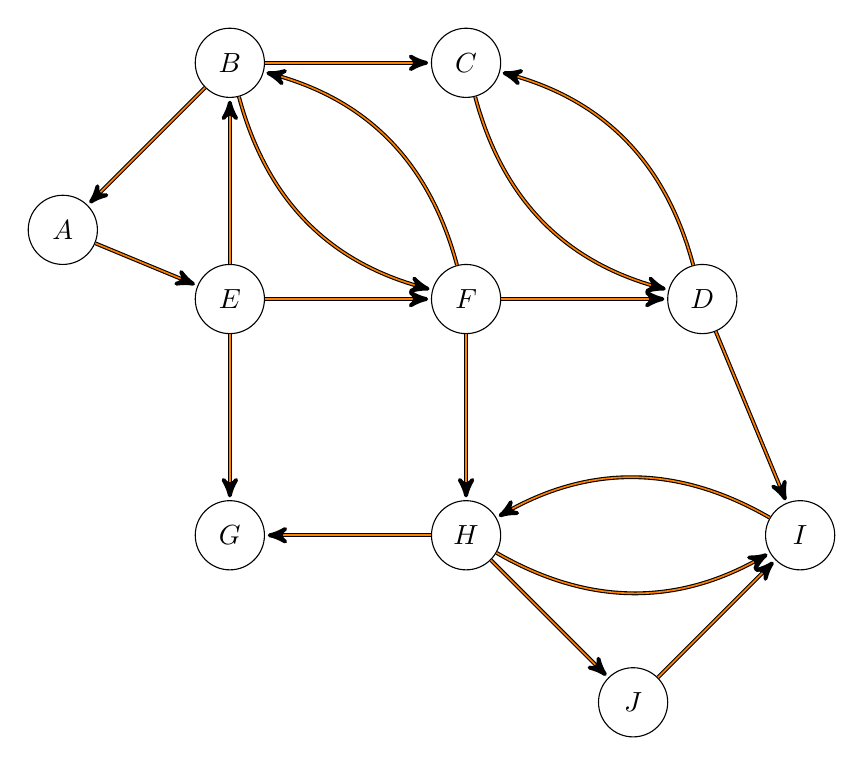
\begin{tikzpicture}[>=stealth',shorten >=1pt,node distance=3cm,on grid,initial/.style    ={}][!hb]
  \node[state]          (A)                        {$A$};
  \node[state]          (B) [above right =of A]    {$B$};
  \node[state]          (C) [right =of B]    {$C$};
  \node[state]          (F) [below =of C]    {$F$};
  \node[state]          (D) [right =of F]    {$D$};
  \node[state]          (E) [below =of B]    {$E$};
  \node[state]          (G) [below =of E]    {$G$};
  \node[state]          (H) [right =of G]    {$H$};
  \node[state]          (J) [below right =of H]   {$J$};
  \node[state]          (I) [above right =of J]    {$I$};
  

\tikzset{mystyle/.style={->,double=orange}} 
\tikzset{every node/.style={fill=white}} 
\path (B)     edge [mystyle] (A)
      (A)     edge [mystyle] (E) 
      (B)     edge [mystyle] (C)
      (B)     edge [bend right] [mystyle] (F)
      (F)     edge [bend right] [mystyle] (B)
      (C)     edge [bend right] [mystyle] (D)
      (D)     edge [bend right] [mystyle] (C)
      (D)     edge [mystyle] (I)
      (E)     edge [mystyle] (B)
      (E)     edge [mystyle] (F)
      (E)     edge [mystyle] (G)
      (F)     edge [mystyle] (D)
      (F)     edge [mystyle] (H)
      (H)     edge [mystyle] (G)
      (J)     edge [mystyle] (I)
      (H)     edge [mystyle] (J)
      (H)     edge [bend right] [mystyle] (I)
      (I)     edge [bend right] [mystyle] (H); 
\end{tikzpicture}
\begin{enumerate}
    \item Give the pre and post number of each vertex in the reverse graph $G^R$.
    \item In what order are the connected components found?
    \item Which are source connected components and which are sink connected components?
    \item Draw the ``metagraph'' (each meta-node is a connected component of $G$).
    \item What is the minimum number of edges you must add to $G$ to make it strongly connected?
\end{enumerate}

\end{qunlist}
\end{document}
